\chapter{Praktische Umsetzung}\label{chp:Umsetzung}
Dieses Kapitel stellt am Beispiel der Lotka-""Volterra-""Form~(LV-Form) ein Konzept 
für die praktische Umsetzung dar.

\section{Lotka-Volterra-Form}
Die Lotka-Volterra-Regeln (LV-Regeln) sind ein Regelwerk "`zur quantitativen Beschreibung 
der Populationsdynamik in Räuber-""Beute-""Beziehungen"' \cite{wikiD:LVR}. Sie wurden 
1925 und 1926 von Alfred Lotka und Vito Volterra formuliert. Die LV-Form ist ein Modell, 
welches auf den LV-Regeln basiert. 

\subsection{Elemente}
Eine LV-Form besteht aus drei Elementen: \emph{Populationen}, \emph{Ereignisse} 
und \emph{Parameter}. Abbildung \ref{pic:LVFKomponenten} stellt diese dar.

%\begin{figure}[htb]
%\centering
%\hspace*{\fill} 
%\subfloat[Population\label{pic:Population}]
%         {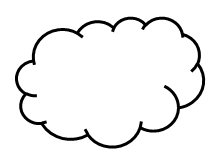
\includegraphics[width=0.2\linewidth,keepaspectratio]{bilder/lvfPopulation}}
%\hspace*{\fill} 
%\subfloat[Ereignis\label{pic:Ereignis}]
%         {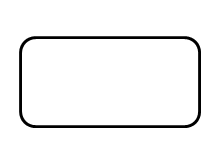
\includegraphics[width=0.2\linewidth,keepaspectratio]{bilder/lvfEreignis}}
%\hspace*{\fill} 
%\subfloat[Parameter\label{pic:Parameter}]
%         {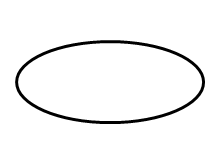
\includegraphics[width=0.2\linewidth,keepaspectratio]{bilder/lvfParameter}}
%\hspace*{\fill} 
%\caption{Elemente der LV-Form}
%\label{pic:LVFKomponenten}
%\end{figure}

\begin{figure}[htb]
\centering
\hspace*{\fill} 
\subfloat[Population\label{pic:Population}]
         {\begin{tikzpicture}
  [thick,
   lvgNode/.style={draw,minimum width=2cm, minimum height=1cm},
   popN/.style={cloud,cloud puffs=9,lvgNode, minimum height=1.5cm},
   parN/.style={ellipse,lvgNode},
   eveN/.style={rectangle,rounded corners=0.25cm,lvgNode},
  ]

 \node[popN] at (0,0) {};
\end{tikzpicture}}
\hspace*{\fill} 
\hspace*{\fill} 
\subfloat[Ereignis\label{pic:Ereignis}]
         {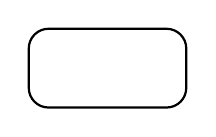
\begin{tikzpicture}
  [thick,
   lvgNode/.style={draw,minimum width=2cm, minimum height=1cm},
   popN/.style={cloud,cloud puffs=9,lvgNode, minimum height=1.5cm},
   parN/.style={ellipse,lvgNode},
   eveN/.style={rectangle,rounded corners=0.25cm,lvgNode},
  ]

 \node[eveN] at (0,0) {};
\end{tikzpicture}}
\hspace*{\fill} 
\hspace*{\fill} 
\subfloat[Parameter\label{pic:Parameter}]
         {\begin{tikzpicture}
  [thick,
   lvgNode/.style={draw,minimum width=2cm, minimum height=1cm},
   popN/.style={cloud,cloud puffs=9,lvgNode, minimum height=1.5cm},
   parN/.style={ellipse,lvgNode},
   eveN/.style={rectangle,rounded corners=0.25cm,lvgNode},
  ]

 \node[parN] at (0,0) {};
\end{tikzpicture}}
\hspace*{\fill} 
\caption{Elemente der LV-Form}
\label{pic:LVFKomponenten}
\end{figure}

\emph{Populationen} sind die Basiselemente. Sie stellen eine Gruppe von Lebewesen dar. 

Ein \emph{Ereignis} ist eine gerichtete Verbindung zweier Populationen miteinander. 
Es kann auch eine Population mit sich selbst verbunden werden. Ereignisse stellen 
Handlungen oder Geschehen in einer Population dar, die Auswirkungen auf die 
Ziel-Population haben.

\emph{Parameter} beeinflussen Ereignisse. Sie sind somit auch immer auf (mindestens) ein 
Ereignis gerichtet. Sie können zusätzlich von Populationen abhängig sein. 

%\begin{figure}[htb]
%\centering
%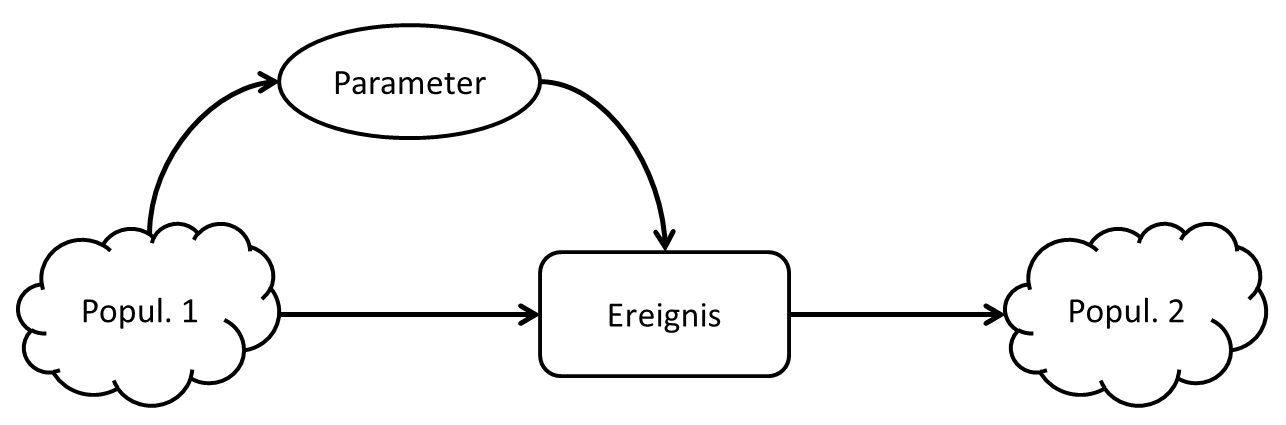
\includegraphics[width=\linewidth,height=\textheight,
%keepaspectratio]{bilder/LVFConns}
%\caption{Mögliche Verbindungen in einer LV-Form}
%\label{pic:LVFConns}
%\end{figure}

\begin{figure}[htb]
\centering
\begin{tikzpicture}
  [thick,node distance=1.5cm,
   lvgNode/.style={draw,minimum width=2cm, minimum height=1cm},
   popN/.style={cloud,cloud puffs=9,lvgNode,shape aspect=1.5,inner sep=-5pt, minimum height=1.5cm},
   parN/.style={ellipse,lvgNode,shape aspect=2},
   eveN/.style={rectangle,rounded corners=0.25cm,shape aspect=2,lvgNode},
  ]

 \node[popN] (pop1)                       {Popul. 1};
 \node[parN] (par)  [above right=of pop1] {Parameter};
 \node[eveN] (eve)  [below right=of par]  {Ereignis};
 \node[popN] (pop2) [right=of eve]        {Popul. 2};

 \draw [->,out=90,in=180] (pop1) to (par);
 \draw [->,out=0,in=90]   (par)  to (eve);
 \draw [->]               (pop1) to (eve);
 \draw [->]               (eve)  to (pop2);
\end{tikzpicture}
\caption{Mögliche Verbindungen in einer LV-Form}
\label{pic:LVFConns}
\end{figure}

\subsection{Formale Umsetzung}
Mit den oben beschriebenen Regeln lässt sich eine LV-Form aus 
Populationen, Ereignissen und Paramtern formal beschreiben.

\begin{mydef}[Lotka-Volterra-Form]\label{def:LVF}
Eine Lotka-Volterra-Form $\Lambda$ ist ein 3-Tupel $\Lambda=(\Pi, \Sigma, 
\Phi)$. Dabei sind:
\begin{itemize}
	\item $\Pi$ eine endliche Menge von Populationen,
	\item $\Sigma \subseteq \Pi \times \Pi$ die Menge an Ereignissen und
	\item $\Phi \subseteq \wp(\Pi) \times (\wp(\Sigma) \backslash \{\emptyset\})$
	      die Menge an Parametern\footnote{$\wp(M)=\{T\ |\ T\subseteq M\}$ ist
	      die Potenzmenge (die Menge aller Teilmengen) von M.}.
\end{itemize}
\end{mydef}

\subsection{Umsetzung als Graph}
Die nun formal beschriebene LV-Form lässt sich auch als Graph umsetzen. Dabei 
sind Populationen, Ereignisse und Parameter jeweils Knoten. Die Kanten ergeben 
sich direkt aus den in Definition \ref{def:LVF} beschrieben Bedingungen. Der 
so entstehende gerichtete Graph sei dann ein Lotka-Volterra-Graph (LVG).

\begin{mydef}[Lotka-Volterra-Graph]
Gegeben sei eine LV-Form $\Lambda=(\Pi, \Sigma, \Phi)$. Der dazugehörige 
gerichtete Lotka-Volterra-Graph $G=(V,E)$ sei wie folgt definiert:

Die Knotenmenge $V$ ist die Vereinigungsmenge der Populationen, Ereignisse 
und Parameter.
\[ V=\Pi \cup \Sigma \cup \Phi \]

Die Kantenmenge $E$ ist die Vereinigung aus der durch Ereignisse erzeugten 
Kantenmenge $E_\Sigma$ sowie der durch Parameter erzeugten Kantenmenge $E_{\Pi\Phi}$ 
und $E_{\Phi\Pi}$. Dabei stellt $E_{\Pi\Phi}$ die Kanten von Populationen zu 
Parametern und $E_{\Phi\Sigma}$ von Parametern zu Ereignissen dar. 
\[ E=E_\Sigma \cup E_{\Pi\Phi} \cup E_{\Phi\Sigma} \]

Für jedes Ereignis $e=(p,q)\in\Sigma$ ist jeweils eine Kante zwischen dem Ereignis 
und den beiden Populationen $p$ und $q$ in $E_\Sigma$ enthalten. 
\[ E_\Sigma=\{(p,e),(e,q)\ |\ e \in \Sigma\} \]

In $E_{\Pi\Phi}$ befindet sich für jeden Parameter $\varphi=(P_\Pi,P_\Sigma) \in \Phi$ 
jeweils eine Kante zwischen den Populationen $\pi \in P_\Pi$ und dem Parameter $\varphi$.
\[ E_{\Pi\Phi}=\bigcup_{\varphi \in \Phi}\{(\pi,\varphi)\ |\ \pi \in P_\Pi\} \]

Des weiteren ist in $E_{\Phi\Sigma}$ für jeden Parameter $\varphi=(P_\Pi,P_\Sigma) \in \Phi$
jeweils eine Kante vom Parameter $\varphi$ zu jedem Ereignis $e \in P_\Sigma$ vorhanden.
\[ E_{\Phi\Sigma}=\bigcup_{\varphi \in \Phi}\{(\varphi,e)\ |\ e \in P_\Sigma\} \]
\end{mydef}

Der so erzeugte LVG lässt sich nun mit anderen Graphen vergleichen.

\section{Veringerung der Komplexität}
Angenommen, eine LV-Form besitzt vier Populationen, pro Population zwei Ereignisse 
und fünf Parameter. Der dazugehörige LVG hat dann 17~Knoten. Vergleicht 
man den LVG mit einem dazu isomorphen Graphen, so gibt es etwa $3{,}6 \cdot 10^{14}$ 
ECGMs. Das B\&B-Verfahren hat in dieser Größenordnung eine hohe Wahrscheinlichkeit 
nicht erfolgreich zu sein. Bei den entsprechenden Tests (Abschnitt \ref{BBTest}) 
mussten die meisten von ihnen abgebrochen werden, weil der Speicherverbrauch zu hoch war. 

\subsection{Vorgabe von Knoten}\label{sec:VorgabeKnoten}
Eine Möglichkeit, die Anzahl der ECGMs zu senken, ist es, dem Lerner Knoten 
vorzugeben. So könnten beispielsweise die Population vorgegeben werden. 
Die entsprechenden Knoten sind dann fest den Populationsknoten in der 
Musterlösung zugeordnet. Die Anzahl der ECGMs sinkt dann auf etwa $6{,}2 \cdot 10^9$. 

Es besteht vermutlich auch die Chance, dass sich durch die Vorgabe schneller deutliche 
Schranken bilden, also dass schneller abgeschätzt werden kann, wie viele Kanten der gemeinsame 
Teilgraph höchstens haben wird. Die Vermutung basiert darauf, dass die zugewiesenen Knoten auch 
Auswirkungen auf die Kanten und somit auf die benachbarten Knoten haben. Gibt es ohne 
Vorgabe beispielsweise für ein verbundenes Paar aus einer Population und einem Ereignis 
vier oder mehr mögliche Abbildungen, so gibt es mit Vorgabe nur noch ein oder zwei. 
Dies liegt daran, dass die Population eindeutig bestimmt werden kann. Somit bleiben 
als mögliche Zuordnungen für das Ereignis nur die Ereignisse der Musterlösung, die 
mit der Population verbunden sind.

\subsection{Knotenfärbung}
Eine weitere Möglichkeit besteht darin, die Knoten eines Graphen in Gruppen zu 
unterteilen, sie zu färben.

\begin{mydef}[Knotenfärbung]
Gegeben sei ein Graph $G=(V,E)$. Eine Knotenfärbung $f$ ist eine Abbildung 
$f: V \rightarrow \mathbb{N}$. Die Farbe eines Knotens $v$ ist dann $f(v)$.
\end{mydef}

Nun erlaubt man in einem ECGM nur Zuweisungen, wenn beide Knoten die gleiche Farbe 
besitzen. Für einen LVG bietet es sich an, die Knoten in drei Farben zu unterteilen: 
je eine Farbe für Populationen, Ereignisse und Parameter. Auch die Vorgabe von Knoten 
lässt sich mittels Färbung umsetzen. Jeder vorgegebene Knoten bekommt eine eigene Farbe. 

Mittels Färbung lässt sich nun die Zahl der möglichen ECGMs von $G_1=(V_1,E_1)$ nach 
$G_2=(V_2,E_2)$ stark reduzieren. Es seien $n_i$ und $m_i$ die Anzahl der Knoten in $G_1$ 
bzw. $G_2$, welche die Farbe $i$ haben.
\begin{align*}
n_i&=\big| \{v\ |\ v \in V_1 \wedge f(v)=i\}\big| \\
m_i&=\big| \{v\ |\ v \in V_2 \wedge f(v)=i\}\big| 
\end{align*}

Es sei dann $p_i$ die Anzahl der ECGMs innerhalb einer Farbe.
\[ p_i=\left\{\begin{array}{ll}
                \frac{n_i!}{(n_i-m_i)!} & n_i \geq m_i \\
                \frac{m_i!}{(m_i-n_i)!} & \text{sonst}
              \end{array}\right. \]
              
Die Gesamtzahl $p$ der ECGMs ist nun das Produkt aller $p_i$.
\[ p=\prod_{i \in \mathbb{N}}p_i \]

Das Beispiel von oben hat dann, wenn es mit einem isomorphen Graphen verglichen wird, 
$4{,}8 \cdot 10^6$ mögliche ECGMs. In der Testreihe des B\&B-Verfahrens, in der die Knoten 
nach Zahl ihrer Nachbarn sortiert wurden (siehe Abbildung \ref{pic:BB_Nh}), wurden alle Tests 
in der Größenordnung von $10^6$ bis $10^7$ Permutationen erfolgreich in unter $1$~Sekunde 
beendet.

\section{Auswertung eines ECGMs}
Nach Ermittlung eines ECGMs ist der nächste Schritt die Auswertung. In der hier vorgestellten 
Variante wird ein Fehlergraph gebildet. Anschließend erfolgt eine Mustersuche auf Basis von
TGI.

\subsection{Fehlergraph}
Die Idee an einem Fehlergraph ist es, dass man beide Graphen zusammenfügt. Zusätzlich 
markiert man die Knoten und Kanten abhängig davon, ob sie hinzugefügt, entfernt oder übernommen 
wurden. Auf diese Weise lässt sich in diesem neuen Graphen nach Mustern suchen. Der so erzeugte Graph 
sei ein Fehlergraph.

\begin{mydef}[Fehlergraph]
Gegeben seien zwei Graphen $G_1=(V_1,E_2)$ und $G_2=(V_2,E_2)$ sowie ein ECGM 
$\varphi:\hat{V}_1 \rightarrow \hat{V}_2$ mit $\hat{V}_1 \subseteq V_1$ und 
$\hat{V}_2 \subseteq V_2$. Aus $G_1$, $G_2$ und $\varphi$ ergeben sich zusätzlich 
$V_d$, $V_a$ $E_d$ und $E_a$ (siehe Abschnitt \ref{sec:Graphabstand}).

Ein Fehlergraph von $G_1$, $G_2$ und $\varphi$ ist dann ein 3-Tupel $F=(V_F,E_F,\alpha)$. 
Dabei sind:
\begin{itemize}
	\item $V_F=V_1 \cup V_a$ die Menge der Knoten,
	\item $E_F=E_1 \cup E_a$ die Menge der Kanten und
	\item $\alpha: V \cup E \rightarrow \{r,g,b\}$ die Markierung der Knoten und Kanten.
\end{itemize}

Dabei wird ein Element des Graphen (ein Knoten oder eine Kante) mit $r$ markiert, 
wenn es entfernt wird. Es erhält $g$ als Markierung, wenn es hinzugefügt wird. 
Ist ein Element in beiden Graphen vorhanden (wird übernommen), dann wird es mit $b$ 
markiert.
\[
\alpha(x)=\left\{\begin{array}{ll}
                    r & x \in V_d \cup E_d \\
                    g & x \in V_a \cup E_a \\
                    b & sonst
                 \end{array}\right.
\]
\end{mydef}

Der so erzeugte Fehlergraph $F$ ist nun ein Graph, der alle Informationen aus den Graphen 
$G_1$ und $G_2$ sowie dem ECGM $\varphi$ enthält. Abbildung \ref{pic:Fehlergraph} stellt dies dar. 
Die Knoten und Kanten sind dabei entsprechend ihrer Markierung in rot, grün und blau 
dargestellt.

%\begin{figure}[htb]
%\centering
%\subfloat[ Eingabe des Lerners\label{pic:FG_Eingabe}]{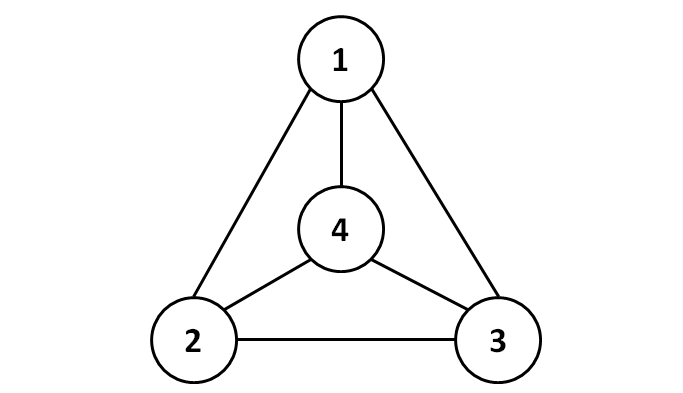
\includegraphics[width=0.4\linewidth,
%keepaspectratio]{bilder/bspFGEingabe}}
%\hspace{1.2cm} 
%\subfloat[Musterlösung\label{pic:FG_Musterloesung}]{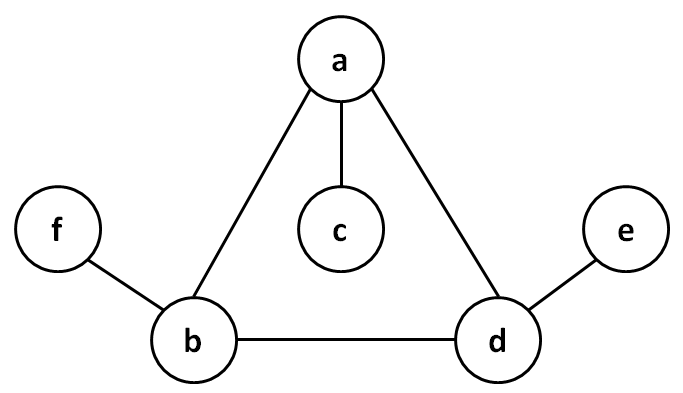
\includegraphics[width=0.4\linewidth,
%keepaspectratio]{bilder/bspFGLsg}}
%\hspace{1.2cm} 
%\subfloat[erzeugter Feh"-ler"-graph\label{pic:FG}]{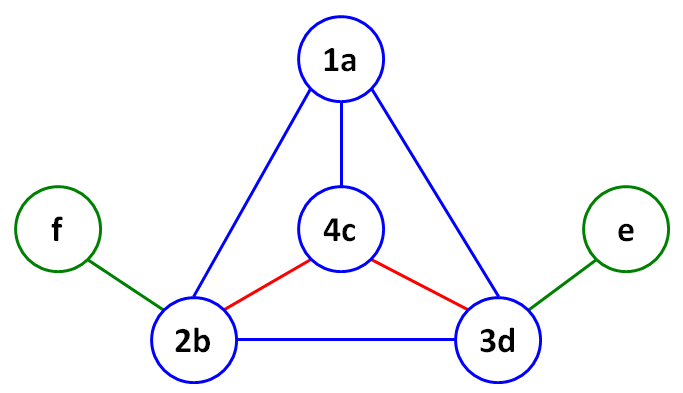
\includegraphics[width=0.4\linewidth,
%keepaspectratio]{bilder/bspFGAusgabe}}
%\caption{Beispiel für einen Fehlergraph}
%\label{pic:Fehlergraph}
%\end{figure}

\begin{figure}[htb]
\centering
\hspace*{\fill} 
\subfloat[Eingabe des Lerners\label{pic:FG_Eingabe}]
{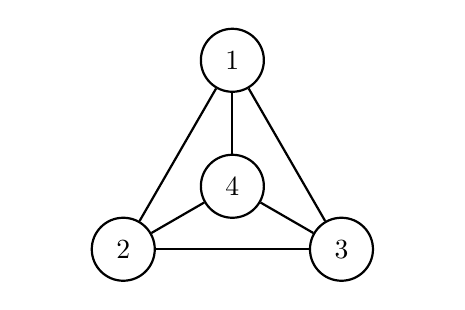
\begin{tikzpicture}
  [normalN/.style={circle,draw,minimum size=0.8cm},
   thick]

  \node[normalN] (c) at   (0:0)   {4};
  \node[normalN] (t) at  (90:1.6) {1};
  \node[normalN] (l) at (210:1.6) {2};
  \node[normalN] (r) at (-30:1.6) {3};
  
  \path (210:1.6)+(120:1.6) node[normalN,black!0] (ll) {};
  \path (-30:1.6)+ (60:1.6) node[normalN,black!0] (rr) {};

  \draw [] (c) -- (t);
  \draw [] (c) -- (l);
  \draw [] (c) -- (r);
  
  \draw [] (t) -- (l);
  \draw [] (t) -- (r);
  \draw [] (l) -- (r);
  
  %\draw [] (l) -- (ll);
  %\draw [] (r) -- (rr);
\end{tikzpicture}}
\hspace*{\fill} 
\subfloat[Musterlösung\label{pic:FG_Musterloesung}]
{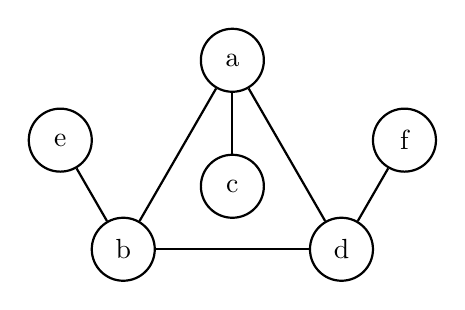
\begin{tikzpicture}
  [normalN/.style={circle,draw,minimum size=0.8cm},
   thick]

  \node[normalN] (c) at   (0:0)   {c};
  \node[normalN] (t) at  (90:1.6) {a};
  \node[normalN] (l) at (210:1.6) {b};
  \node[normalN] (r) at (-30:1.6) {d};
  
  \path (210:1.6)+(120:1.6) node[normalN] (ll) {e};
  \path (-30:1.6)+ (60:1.6) node[normalN] (rr) {f};

  \draw [] (c) -- (t);
  %\draw [] (c) -- (l);
  %\draw [] (c) -- (r);
  
  \draw [] (t) -- (l);
  \draw [] (t) -- (r);
  \draw [] (l) -- (r);
  
  \draw [] (l) -- (ll);
  \draw [] (r) -- (rr);
\end{tikzpicture}}
\hspace*{\fill} \\ \hspace*{\fill} 
\subfloat[erzeugter Feh"-ler"-graph\label{pic:FG}]
{\begin{tikzpicture}
  [normalN/.style={circle,draw,minimum size=0.8cm},
   thick,draw=blue]

  \node[normalN] (c) at   (0:0)   {4c};
  \node[normalN] (t) at  (90:1.6) {1a};
  \node[normalN] (l) at (210:1.6) {2b};
  \node[normalN] (r) at (-30:1.6) {3d};
  
  \path (210:1.6)+(120:1.6) node[normalN,draw=darkgreen] (ll) {e};
  \path (-30:1.6)+ (60:1.6) node[normalN,draw=darkgreen] (rr) {f};

  \draw [] (c) -- (t);
  \draw [red] (c) -- (l);
  \draw [red] (c) -- (r);
  
  \draw [] (t) -- (l);
  \draw [] (t) -- (r);
  \draw [] (l) -- (r);
  
  \draw [darkgreen] (l) -- (ll);
  \draw [darkgreen] (r) -- (rr);
\end{tikzpicture}}
\hspace*{\fill} 
\caption{Beispiel für einen Fehlergraph}
\label{pic:Fehlergraph}
\end{figure}

\subsection{Mustererkennung}
Das Erkennen von Mustern in einem Fehlergraphen lässt sich über Teilgraphisomorphie (TGI) realisieren. 
Dabei stellt man die Muster als Graphen dar, zu denen dann isomorphe Teilgraphen im 
Fehlergraphen gesucht werden. Zwar ist TGI auch NP-vollständig, ein Muster ist aber 
höchstens so groß wie der Fehlergraph. Nimmt man zusätzlich an, dass die gesuchten Muster 
deutlich kleiner sind als die Fehlergraphen, so sollte selbst mit einfachen Algorithmen wie 
Backtracking die Laufzeit in verträglichem Maße bleiben.

\subsubsection{Elementare Muster}
Die zu suchenden Muster sind Graphen. Ihre Elemente sind Knoten und Kanten. Somit stellt 
ein Knoten bzw. eine Kante ein elementares Muster dar. Dabei ist vor allem die Markierung 
interessant. Die drei bei Fehlergraphen verwendeten Markierungen lassen sich erweitern. 
So wäre es eine Möglichkeit, Knoten und Kanten mit beliebiger Markierung zuzulassen. 
Abbildung \ref{pic:bspElementareMuster} stellt mögliche elementare Varianten für Knoten dar. Ist eine 
beliebige Markierung zulässig, so wird der Knoten gestrichelt gezeichnet. Kanten verhalten 
sich dazu analog.

Dieses Prinzip lässt sich auch auf die Färbung von Knoten erweitern. So ist es denkbar, 
dass man in dem Fehlergraphen eines LVG etwas sucht. Ein elementares Muster wäre hier, 
dass ein Ereignis entfernt wird (Abbildung~\ref{pic:bspEreignisLoeschen}).

%\begin{figure}[htb]
%\centering
%\hspace*{\fill} 
%\subfloat[belibiger Knoten\label{pic:bspBelibiegerKnoten}]
%         {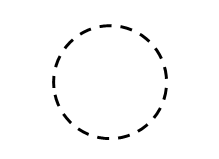
\includegraphics[width=0.2\linewidth,keepaspectratio]{bilder/bspBelibiegerKnoten}}
%\hspace*{\fill} 
%\subfloat[entferntes Ereignis\label{pic:bspEreignisLoeschen}]
%         {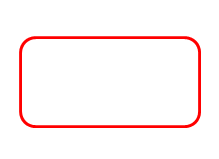
\includegraphics[width=0.2\linewidth,keepaspectratio]{bilder/bspEreignisLoeschen}}
%\hspace*{\fill} 
%\subfloat[gemeinsame Population\label{pic:bspGemeinsamePopulation}]
%         {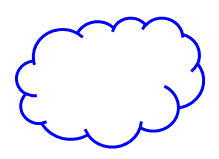
\includegraphics[width=0.2\linewidth,keepaspectratio]{bilder/bspGemeinsamePopulation}}
%\hspace*{\fill} 
%\caption{Beispiele für elementare Knotenmuster}
%\label{pic:bspElementareMuster}
%\end{figure}

\begin{figure}[htb]
\centering
\hspace*{\fill} 
\subfloat[beliebiger Knoten\label{pic:bspBelibiegerKnoten}]
         {\begin{tikzpicture}
  [thick,
   lvgNode/.style={draw,minimum width=2cm, minimum height=1cm},
   normalN/.style={draw,minimum size=1.25cm,circle},
   popN/.style={cloud,cloud puffs=9,lvgNode, minimum height=1.5cm},
   parN/.style={ellipse,lvgNode},
   eveN/.style={rectangle,rounded corners=0.25cm,lvgNode},
  ]

 \node[normalN,dashed] at (0,0) {};
 \node[minimum width=3cm, minimum height=1.5cm] at (0,0) {};
\end{tikzpicture}}
\hspace*{\fill} 
\hspace*{\fill} 
\subfloat[entferntes Ereignis\label{pic:bspEreignisLoeschen}]
         {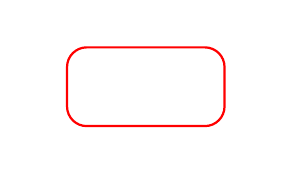
\begin{tikzpicture}
  [thick,
   lvgNode/.style={draw,minimum width=2cm, minimum height=1cm},
   normalN/.style={draw,minimum size=1.25cm,circle},
   popN/.style={cloud,cloud puffs=9,lvgNode, minimum height=1.5cm},
   parN/.style={ellipse,lvgNode},
   eveN/.style={rectangle,rounded corners=0.25cm,lvgNode},
  ]

 \node[eveN,red] at (0,0) {};
 \node[minimum width=3cm, minimum height=1.5cm] at (0,0) {};
\end{tikzpicture}}
\hspace*{\fill} 
\hspace*{\fill} 
\subfloat[gemeinsame Population\label{pic:bspGemeinsamePopulation}]
         {\begin{tikzpicture}
  [thick,
   lvgNode/.style={draw,minimum width=2cm, minimum height=1cm},
   normalN/.style={draw,minimum size=1.25cm,circle},
   popN/.style={cloud,cloud puffs=9,lvgNode, minimum height=1.5cm},
   parN/.style={ellipse,lvgNode},
   eveN/.style={rectangle,rounded corners=0.25cm,lvgNode},
  ]

 \node[popN,blue] at (0,0) {};
 \node[minimum width=2.3cm, minimum height=1.5cm] at (0,0) {};
\end{tikzpicture}}
\hspace*{\fill} 
\caption{Beispiele für elementare Knotenmuster}
\label{pic:bspElementareMuster}
\end{figure}

\subsubsection{Einfache Muster}
Mittels der elementaren Muster lassen sich nun größere Muster entwerfen. So lässt 
sich mit dem Muster in Abbildung \ref{pic:bspKnotenZuViel} beispielsweise erkennen, dass der 
Lerner lediglich einen Knoten zu viel hinzugefügt hat. Betrachtet 
man nur die Zahl der entfernten und hinzugefügten Knoten, so würde man dem Lerner 
zwei überflüssige Kanten, einen überflüssigen Knoten 
und eine fehlende Kante anlasten. Das Muster ermöglicht somit eine andere Bewertung.

%\begin{figure}[htb]
%\centering
%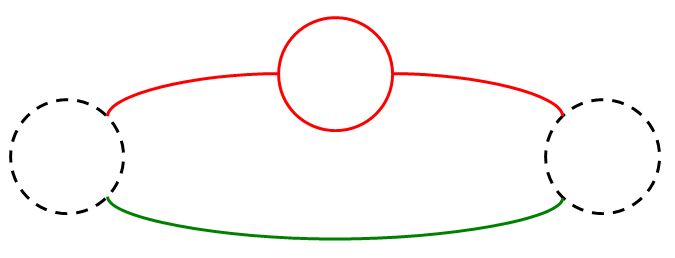
\includegraphics[width=0.7\linewidth,height=\textheight,
%keepaspectratio]{bilder/bspKnotenZuViel}
%\caption{Knoten zu viel}
%\label{pic:bspKnotenZuViel}
%\end{figure}

\begin{figure}[htb]
\centering
\begin{tikzpicture}
  [thick,node distance=5cm,
   lvgNode/.style={draw,minimum width=2cm, minimum height=1cm},
   normalN/.style={draw,minimum size=1.25cm,circle},
   popN/.style={cloud,cloud puffs=9,lvgNode, minimum height=1.5cm},
   parN/.style={ellipse,lvgNode},
   eveN/.style={rectangle,rounded corners=0.25cm,lvgNode},
  ]

 \node[normalN,dashed] (l) {};
 \node[normalN,dashed] (r) [right=of l] {};
 
 \draw[out=45,in=135,red]       (l) .. controls +(45:2cm) and +(135:2cm) ..
                                       node [normalN,fill=white] {}         (r);

 \draw[darkgreen] (l) .. controls +(-45:2cm) and +(-135:2cm) .. (r);

\end{tikzpicture}
\caption{Knoten zu viel}
\label{pic:bspKnotenZuViel}
\end{figure}

Die Abbildungen \ref{pic:bspFalscheRichtung} und \ref{pic:bspFalschePopulation} zeigen zwei 
weitere Beispiele. Im ersten Fall wurde 
eine Kante in die falsche Richtung eingetragen. Das zweite Beispiel verwendet zusätzlich 
die Knotenfärbung. Es gibt an, dass ein Ereignis auf die falsche Population gerichtet ist.

%\begin{figure}[htb]
%\centering
%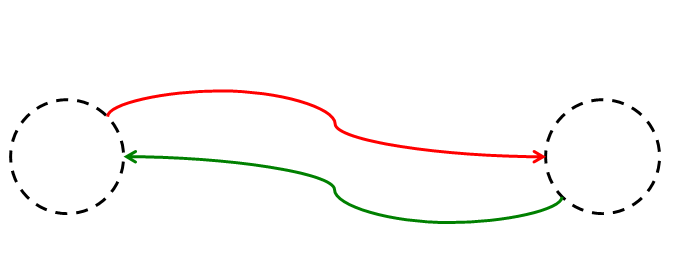
\includegraphics[width=0.7\linewidth,height=\textheight,
%keepaspectratio]{bilder/bspFalscheRichtung}
%\caption{Falsche Richtung einer Kante}
%\label{pic:bspFalscheRichtung}
%\end{figure}

\begin{figure}[htb]
\centering
\begin{tikzpicture}
  [thick,node distance=5cm,
   lvgNode/.style={draw,minimum width=2cm, minimum height=1cm},
   normalN/.style={draw,minimum size=1.25cm,circle},
   popN/.style={cloud,cloud puffs=9,lvgNode, minimum height=1.5cm},
   parN/.style={ellipse,lvgNode},
   eveN/.style={rectangle,rounded corners=0.25cm,lvgNode},
  ]

 \node[normalN,dashed] (l) {};
 \node[normalN,dashed] (r) [right=of l] {};
 
 \draw[->,out=45,in=180,red]       (l) to (r);
 \draw[<-,out=0,in=-135,darkgreen] (l) to (r);

\end{tikzpicture}
\caption{Falsche Richtung einer Kante}
\label{pic:bspFalscheRichtung}
\end{figure}

%\begin{figure}[htb]
%\centering
%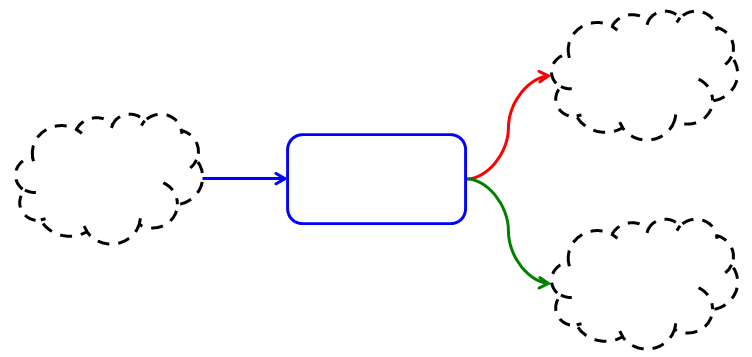
\includegraphics[width=0.7\linewidth,height=\textheight,
%keepaspectratio]{bilder/bspFalschePopulation}
%\caption{Ereignis zielt auf falsche Population}
%\label{pic:bspFalschePopulation}
%\end{figure}

\begin{figure}[htb]
\centering
\begin{tikzpicture}
  [thick,node distance=3cm,
   lvgNode/.style={draw,minimum width=2cm, minimum height=1cm},
   normalN/.style={draw,minimum size=1.25cm,circle},
   popN/.style={cloud,cloud puffs=9,lvgNode, minimum height=1.5cm},
   parN/.style={ellipse,lvgNode},
   eveN/.style={rectangle,rounded corners=0.25cm,lvgNode},
  ]

 \node[popN,dashed] (pl)  at (-3.5,0)    {};
 \node[eveN,blue]   (ev)  at    (0,0)    {};
 \node[popN,dashed] (prt) at  (3.5,1.2)  {};
 \node[popN,dashed] (prb) at  (3.5,-1.2) {};
 
 \draw[->,blue]                   (pl) to (ev);
 \draw[->,out=0,in=180,darkgreen] (ev) to (prb);
 \draw[->,out=0,in=180,red]       (ev) to (prt);

\end{tikzpicture}
\caption{Ereignis zielt auf falsche Population}
\label{pic:bspFalschePopulation}
\end{figure}

\subsubsection{Musterhierarchie}
Bildet man aus einfachen Mustern größere, so entsteht dabei auch eine Hierarchie. Das 
Erkennen dieser Hierarchie kann Vorteile für die Suche nach Mustern und die Bewertung der 
Eingabe des Lerners haben.

Ist ein kleines Muster Teil eines größeren, so hat dies zur Folge, dass das größere 
nur dann vorhanden ist, wenn auch das kleinere gefunden wurde. Mit einer Hierachie 
lässt sich somit der Aufwand für die Mustersuche verringern, indem zuerst kleinere Muster 
gesucht werden. Wurde ein kleineres Muster nicht gefunden, so ist auch kein Muster im 
Fehlergraphen enthalten, welches sich aus dem kleinen ergibt. Zusätzlich dienen bereits 
gefundene kleine Muster als Suchgrundlage für die Großen. Es ist somit nicht mehr nötig, 
den gesamten Fehlergraphen zu durchsuchen.

Für die Bewertung der Lerner-Eingabe kann eine Hierachie dann hilfreich sein, wenn große und 
kleine Muster gefunden werden. Ist ein größeres Muster im Fehlergraph vorhanden, so sind 
dies auch kleinere Muster, wenn sie Teil des größeren sind. Werden nun das große und das 
kleinere Muster bewertet, fließen die kleineren Muster mehrfach in die Bewertung ein. Dies 
mag nicht immer erwünscht sein.


\subsubsection{Berechnung der Hierarchie}
Das Ermitteln der Hierarchie erfolgt erneut über TGI. Dabei wird überprüft, ob ein Muster 
ein Teilgraph eines anderen ist. Auf diese Weise baut sich ein gerichteter azyklischer Graph 
(engl. directed acyclic graph; kurz DAG) auf. Dabei stellt jeder Knoten ein Muster dar. 
Existiert ein Pfad von einem Knoten $u$ zu einem Knoten $v$, dann ist das Muster von $u$ 
ein Teilgraph des Musters von $v$.

Geht man davon aus, dass das Überprüfen der TGI in 
$\mO(\tau)$ möglich ist und es insgesamt $n$ Muster gibt, dann lässt sich der DAG in 
$\mO(n^2\tau)$ bilden. Dazu stellt man den DAG als Adjazenzmatrix der Größe $n\times n$ dar. 
Das Element $(i,j)$ der Matrix hat dann den Wert $0$, wenn es keine Kante gibt oder $i=j$, 
und den Wert $1$, wenn es eine Kante gibt, also wenn Muster $i$ Teilgraph von Muster $j$ ist.

Wenn erwünscht, kann man redundante Kanten auch entfernen. Eine Kante $(i,j)$ ist redundant 
genau dann, wenn es einen Knoten (ein Muster) $k$ gibt, und ein Pfad von $i$ über $k$ zu $j$ 
existiert. Um redundante Kanten zu entfernen muss man nun einfach alle paarweise verschiedenen 
$i$, $j$, und $k$ überprüfen. Da sich dies einfach aus der Adjazenzmatrix auslesen lässt, ergibt 
sich somit ein zusätzlicher Aufwand von $\mO(n^3)$. Um das Übersehen redundanter Kanten aufgrund 
von bereits entfernten zu vermeiden, sollten Kanten jedoch erstmal nur zum Löschen markiert  
und im Nachhinein gelöscht werden.

\begin{figure}[htb]
\centering
\begin{tikzpicture}
  [normalN/.style={circle,draw,minimum size=0.8cm,thick},
   node distance=0.8cm]

       
  \node[normalN] (i) {i};
  \node[normalN] (k) [above right=of i] {k};
  \node[normalN] (j) [below right=of k] {j};

  \draw [thick,->,dashed] (i) -- (j);
  \draw [thick,->] (i) -- (k);
  \draw [thick,->] (k) -- (j);
      
\end{tikzpicture}\caption{Redundante Kante $(i,j)$ in der Musterhierarchie}
\label{pic:bsp_redunEdge}
\end{figure}

Der gesamte Aufwand liegt 
dann höchstens bei $\mO(n^2\tau + n^3)$. Insgesamt ist der Aufwand jedoch nebensächlich, 
denn die Hierarchie lässt sich bereits beim Entwurf einer Aufgabe ermitteln. Es ist nicht 
nötig dies bei jeder Eingabe des Lerners zu wiederholen.

\subsubsection{Überschneidung von Mustern}
Eine Problematik, die man bei der Mustersuche beachten muss, ist die 
Überschneidung von Mustern. Zwei Muster können einen gemeinsamen 
Teilgraphen besitzen. Werden nun beide Muster erkannt, kann es 
vorkommen, dass sie sich überschneiden. Dies kann zu einer fehlerhaften 
Bewertung führen. Erkennen lässt sich ein gemeinsamer Teilgraph indem 
man das ECGM für beide Muster ermittelt.

Prinzipiell bieten sich drei Varianten für den Umgang mit Musterüberschneidungen an:
\begin{itemize}

	\item \textbf{Ignorieren:} Sollte eine Überschneidung keine relevanten 
	      Folgen haben, so ist die Suche auch nicht nötig.
	      
	\item \textbf{Nachträgliche Suche:} Zuerst werden alle Muster im Fehlergraphen 
	      ermittelt. Erst danach wird überprüft, ob es zu Überschneidungen gekommen 
	      ist.

	\item \textbf{Sperren von Knoten:} Legt man fest, dass ein Knoten bzw. eine 
	      Kante nur zu einem Muster gehören kann, dann schließt man damit 
	      Überschneidungen aus. Dabei sollte man jedoch auf die Reihenfolge 
	      achten, mit der man nach Mustern sucht. Es kann passieren, dass ein 
	      weniger wichtiges Muster zuerst gefunden wird und somit ein wichtiges Muster 
	      sperrt.
\end{itemize}

